\documentclass[tikz,border=10pt]{standalone}
\usepackage{tikz}
\usetikzlibrary{arrows.meta,shapes.geometric}

\tikzset{>=Latex}

\begin{document}
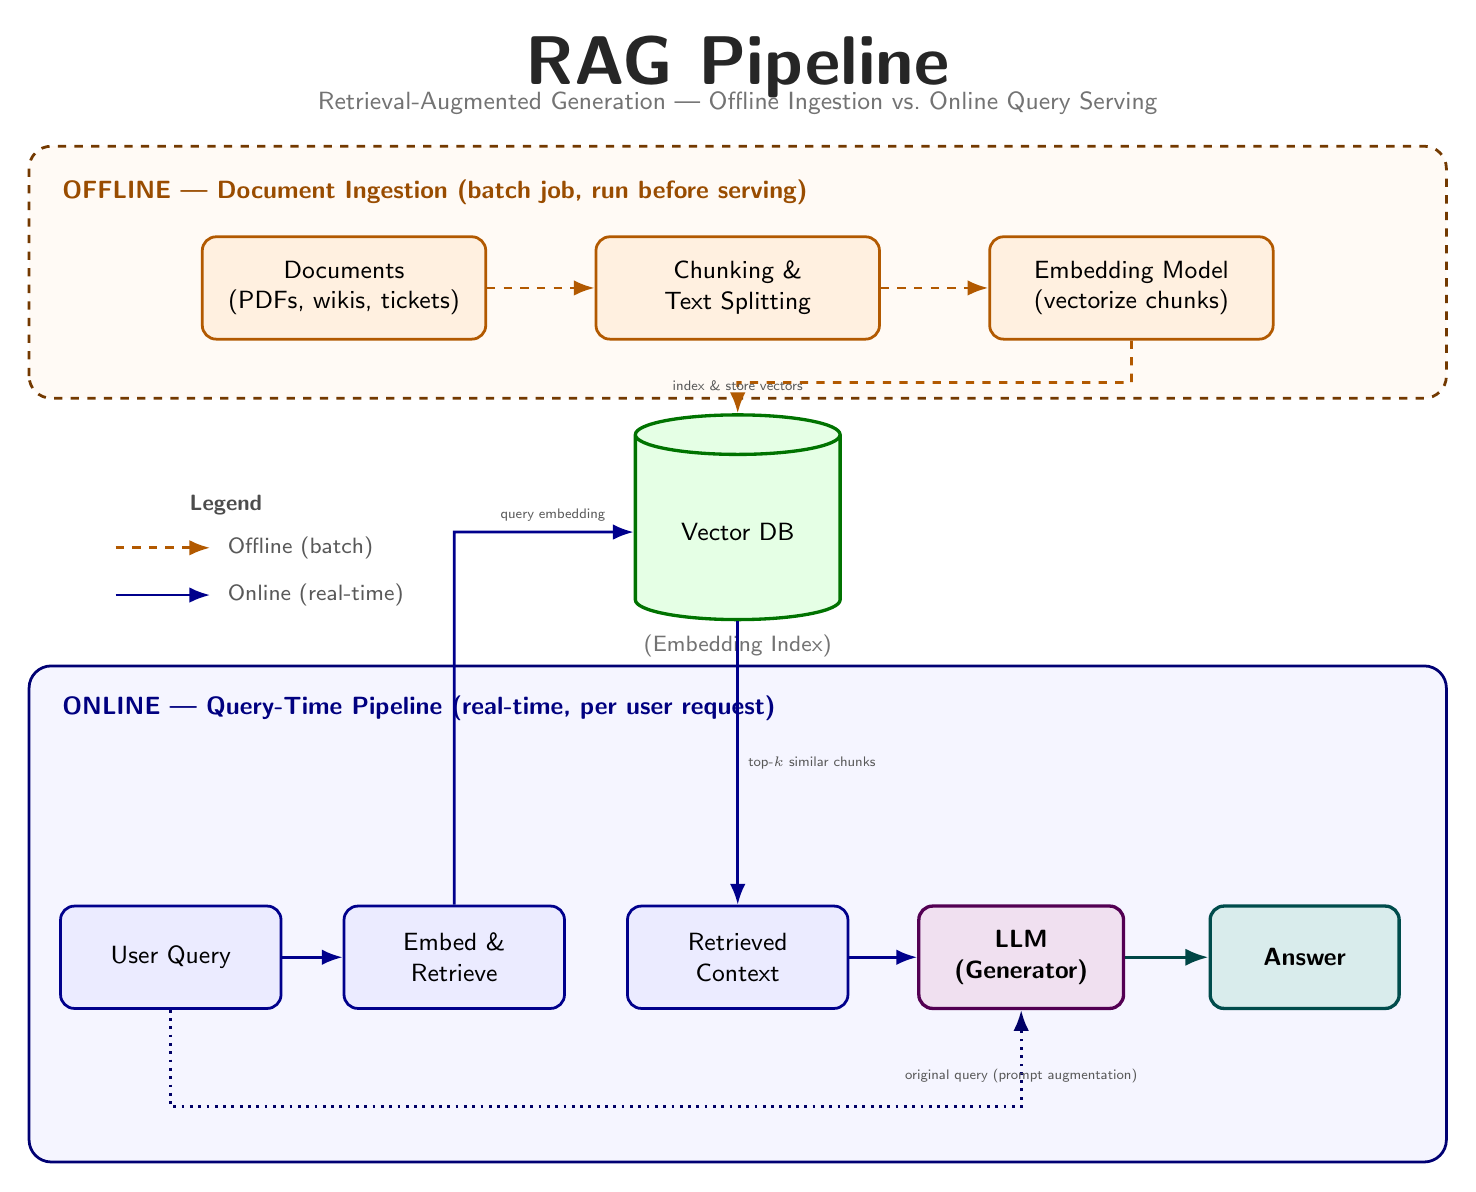
\begin{tikzpicture}[
  offlinebox/.style={rectangle, rounded corners=5pt, draw=orange!70!black, fill=orange!12,
    line width=1pt, minimum width=3.6cm, minimum height=1.3cm, align=center,
    font=\sffamily\small, inner sep=4pt},
  onlinebox/.style={rectangle, rounded corners=5pt, draw=blue!55!black, fill=blue!8,
    line width=1pt, minimum width=2.8cm, minimum height=1.3cm, align=center,
    font=\sffamily\small, inner sep=4pt},
  llmbox/.style={rectangle, rounded corners=5pt, draw=violet!65!black, fill=violet!12,
    line width=1.2pt, minimum width=2.6cm, minimum height=1.3cm, align=center,
    font=\sffamily\bfseries\small, inner sep=4pt},
  ansbox/.style={rectangle, rounded corners=5pt, draw=teal!60!black, fill=teal!15,
    line width=1.2pt, minimum width=2.4cm, minimum height=1.3cm, align=center,
    font=\sffamily\bfseries\small, inner sep=4pt},
  vdbstyle/.style={cylinder, shape border rotate=90, aspect=0.3, draw=green!45!black,
    fill=green!10, line width=1.2pt, minimum width=2.6cm, minimum height=2.6cm,
    align=center, font=\sffamily\small},
  offlinearrow/.style={->, dashed, line width=1pt, color=orange!70!black},
  onlinearrow/.style={->, line width=1pt, color=blue!55!black},
  queryarrow/.style={->, dotted, line width=1pt, color=blue!40!black},
  ansarrow/.style={->, line width=1.2pt, color=teal!55!black},
  lbl/.style={font=\sffamily\tiny, text=black!65}
]

% ---------- Lane backgrounds ----------
\draw[rounded corners=8pt, draw=orange!45!black, dashed, line width=1pt, fill=orange!4]
  (0.5,10.1) rectangle (18.5,13.3);
\draw[rounded corners=8pt, draw=blue!45!black, line width=1pt, fill=blue!4]
  (0.5,0.4) rectangle (18.5,6.7);

% ---------- Titles ----------
\node[font=\sffamily\bfseries\Huge, text=black!85] at (9.5,14.3) {RAG Pipeline};
\node[font=\sffamily\small, text=black!55] at (9.5,13.85)
  {Retrieval-Augmented Generation --- Offline Ingestion vs.\ Online Query Serving};

\node[anchor=north west, font=\sffamily\bfseries\small, text=orange!60!black] at (0.8,13.0)
  {OFFLINE --- Document Ingestion (batch job, run before serving)};
\node[anchor=north west, font=\sffamily\bfseries\small, text=blue!50!black] at (0.8,6.45)
  {ONLINE --- Query-Time Pipeline (real-time, per user request)};

% ---------- Offline nodes ----------
\node[offlinebox] (docs) at (4.5,11.5) {Documents\\(PDFs, wikis, tickets)};
\node[offlinebox] (chunk) at (9.5,11.5) {Chunking \&\\Text Splitting};
\node[offlinebox] (embedm) at (14.5,11.5) {Embedding Model\\(vectorize chunks)};

% ---------- Vector DB ----------
\node[vdbstyle] (vdb) at (9.5,8.4) {Vector DB};
\node[font=\sffamily\footnotesize, text=black!55] at (9.5,6.95) {(Embedding Index)};

% ---------- Online nodes ----------
\node[onlinebox] (uq) at (2.3,3.0) {User Query};
\node[onlinebox] (er) at (5.9,3.0) {Embed \&\\Retrieve};
\node[onlinebox] (rc) at (9.5,3.0) {Retrieved\\Context};
\node[llmbox] (llm) at (13.1,3.0) {LLM\\(Generator)};
\node[ansbox] (ans) at (16.7,3.0) {Answer};

% ---------- Offline flow arrows ----------
\draw[offlinearrow] (docs.east) -- (chunk.west);
\draw[offlinearrow] (chunk.east) -- (embedm.west);
\draw[offlinearrow] (embedm.south) -- (14.5,10.3) -- (9.5,10.3) -- (vdb.north)
  node[lbl, pos=0.62, above] {index \& store vectors};

% ---------- Online flow arrows ----------
\draw[onlinearrow] (uq.east) -- (er.west);
\draw[onlinearrow] (er.north) -- (5.9,8.4) -- (vdb.west)
  node[lbl, pos=0.55, above] {query embedding};
\draw[onlinearrow] (vdb.south) -- (rc.north)
  node[lbl, pos=0.5, right] {top-$k$ similar chunks};
\draw[onlinearrow] (rc.east) -- (llm.west);
\draw[ansarrow] (llm.east) -- (ans.west);

% ---------- Direct query passthrough (prompt augmentation) ----------
\draw[queryarrow] (uq.south) -- (2.3,1.1) -- (13.1,1.1) -- (llm.south)
  node[lbl, pos=0.5, below] {original query (prompt augmentation)};

% ---------- Legend ----------
\node[font=\sffamily\bfseries\footnotesize, text=black!70] at (3.0,8.75) {Legend};
\draw[offlinearrow] (1.6,8.2) -- (2.8,8.2);
\node[anchor=west, font=\sffamily\footnotesize, text=black!65] at (2.9,8.2) {Offline (batch)};
\draw[onlinearrow] (1.6,7.6) -- (2.8,7.6);
\node[anchor=west, font=\sffamily\footnotesize, text=black!65] at (2.9,7.6) {Online (real-time)};

\end{tikzpicture}
\end{document}
